\documentclass[12pt,final,oneside]{article} % use larger type; default would be 10pt
\usepackage{etex}
\usepackage[utf8]{inputenc} % set input encoding (not needed with XeLaTeX)
\usepackage[margin=2cm]{geometry}
\usepackage{xy}
\usepackage{amsmath, amsthm}
\usepackage{showkeys}
\usepackage[smaller]{acronym}
\usepackage[marginclue]{fixme}
%\usepackage{natbib}
\usepackage{tabularx}
\usepackage{chngpage}
\usepackage{booktabs}
\usepackage{cite}
\usepackage{times}
\usepackage{graphicx}
\usepackage{ctable}
\usepackage{footnote}
\usepackage{amssymb}
\usepackage{url}
\usepackage{tikz-timing}
\usepackage[lofdepth,lotdepth]{subfig}
\usepackage{multirow}
\usepackage{tameflts}
\usepackage{algpseudocode}
\usepackage{algorithm}
\usepackage{placeins}
\usepackage{hyperref}
\fxsetup{
    status=draft,
    author=,
    layout=marginclue,inline, % also try footnote or pdfnote
    theme=color
}
\definecolor{fxnote}{rgb}{0.8000,0.0000,0.0000}

\setcounter{tocdepth}{3}

\usepackage{color}
\usepackage[final]{listings}
\lstset{ %
language=C++,                % choose the language of the code
basicstyle=\ttfamily,       % the size of the fonts that are used for the code
numbers=left,                   % where to put the line-numbers
numberstyle=\footnotesize,      % the size of the fonts that are used for the line-numbers
stepnumber=1,                   % the step between two line-numbers. If it is 1 each line will be numbered
numbersep=5pt,                  % how far the line-numbers are from the code
backgroundcolor=\color{white},  % choose the background color. You must add \usepackage{color}
showspaces=false,               % show spaces adding particular underscores
showstringspaces=false,         % underline spaces within strings
showtabs=false,                 % show tabs within strings adding particular underscores
frame=single,           % adds a frame around the code
tabsize=2,          % sets default tabsize to 2 spaces
captionpos=b,           % sets the caption-position to bottom
breaklines=false,        % sets automatic line breaking
breakatwhitespace=false,    % sets if automatic breaks should only happen at whitespace
escapeinside={\%*}{*)}          % if you want to add a comment within your code
}
\begin{document}
   \section{TODO!!!!!!!!!!!!!!!!!!}
      Higher level description.
      Explain non-intuitive operations at the level of the algorithm below it.
      queue.Dequeue -> intuitive, described that it's a FIFO queue.
      CutLoops -> One line description of input -> output, not specifics of how. See Algorithm number for details.
      Repeat high level description for algorithm before.
      See section blah for a discussion of the recovery time calculation
      Explain WriteToFile - Just outputting 


\section{Data Structures}
\subsection{Basic Types}
The following are the basic types, out of which others are built, and which will be referred to. There is generally, but not always, a direct relationship to a C++ primitive.
\\
        \begin{tabularx}{\linewidth}{XXX}
        \toprule
        Name & Closest C++ Equivalent & Description\\
        \midrule
        Integer &  int & Whole number \\
        Float & float & Floating point number \\
        Queue & std::list & FIFO queue \\
        List(type) & std::list$\langle$type$\rangle$ &\\
        String & std::string & String object that provides operations to manipulate itself \\
        File & std::iostream & Abstract type to represent simple I/O operations \\
        Map(KeyType $\to$ ValueType, DEFAULT:  DefaultValue) & std::unordered\_map$\langle$KeyType, ValueType$\rangle$ & A map to translate values of type KeyType to values of type ValueType. If the key isn't present, returns DefaultValue \\
        \bottomrule
        \end{tabularx}
\\
\\
The following are complex types, which are further defined below. This is merely a quick description of each.
\\
        \begin{tabularx}{\linewidth}{lX}
        \toprule
        Name & Description\\
        \midrule
        Blif & Parent object, contains all information about a BLIF file and provides useful operations \\
        BlifModel & Represents a circuit within a BLIF file, and provides methods to manipulate said circuit \\
        BlifNode & A circuit element, or node in the DFG representing the circuit \\
        Signal & A signal within a specific circuit, or BlifModel, representing a set of edges with common source \\
        \bottomrule
        \end{tabularx}

   \begin{figure}
      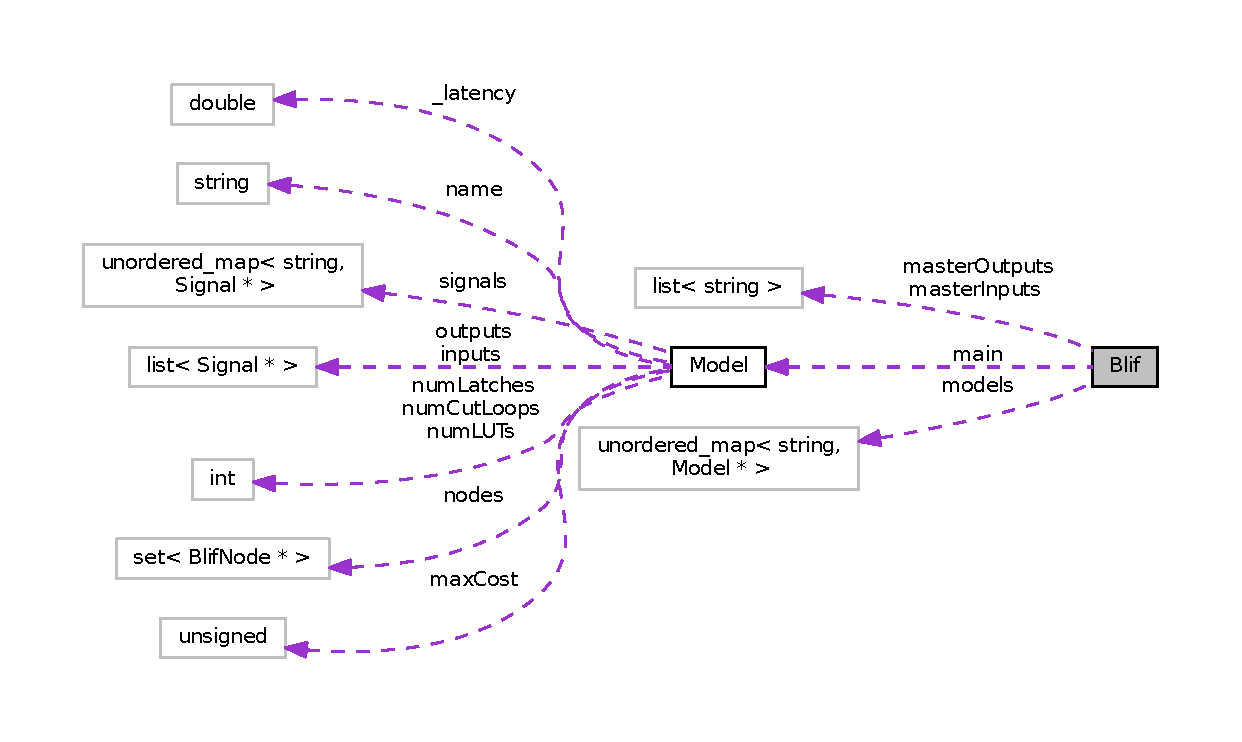
\includegraphics{doxygen/classBlif__coll__graph.pdf}
   \end{figure}
   \begin{figure}
      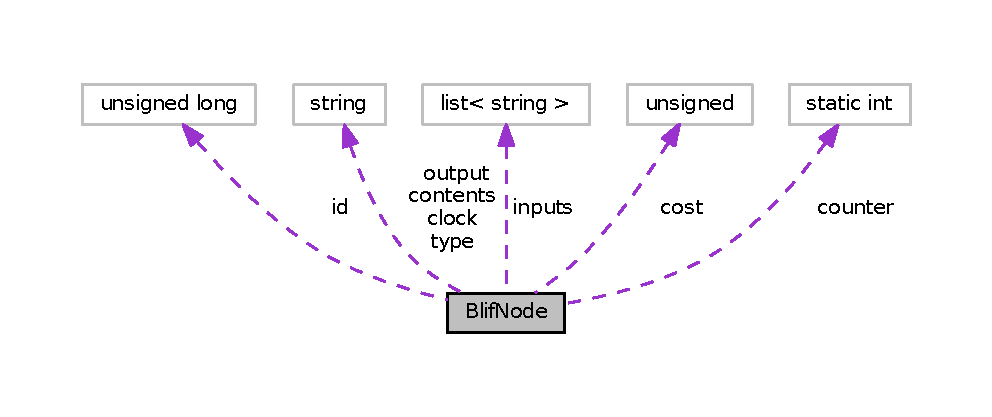
\includegraphics{doxygen/classBlifNode__coll__graph.pdf}
   \end{figure}
   \begin{figure}
      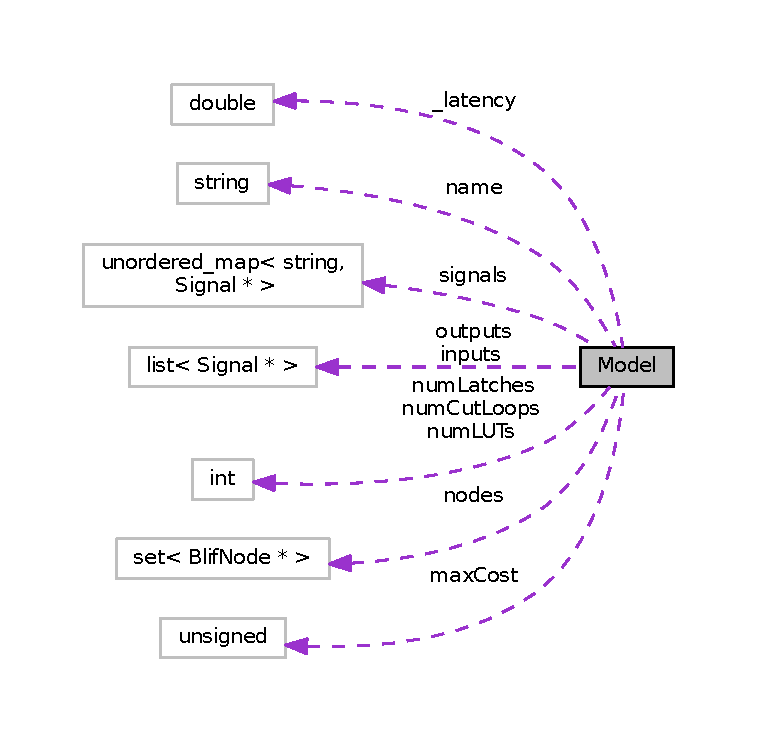
\includegraphics{doxygen/classModel__coll__graph.pdf}
   \end{figure}
   \begin{figure}
      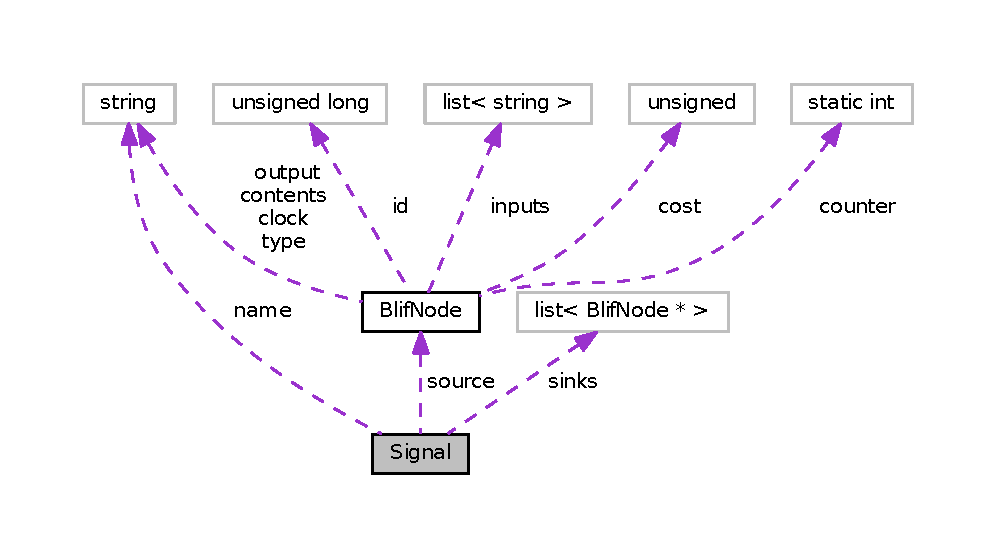
\includegraphics{doxygen/classSignal__coll__graph.pdf}
   \end{figure}

   \subsection{Blif}
      
   \subsection{Model}
      Represents the circuit as a DFG. Contains a list of nodes, map of signal name $\to$ Signal*, and lists of primary inputs and outputs for the circuit.
      Each node contains the names of its input and output signals, allowing the Signal* to be looked up, then the Signal* contains pointers to its source and sink nodes.
      This allows the DFG to be traversed by going from node, to signal, to node, etc.
      The reason for having signals be referred to by name and looked up, rather than a node pointing directly to a signal is twofold.
      One, a node is an independent construct which can be added to or removed from any Model*. For example, when adding a node into a partition. Signals, on the other hand, are circuit specific and are created and destroyed as circumstances demand.
      Two, regardless of implementation, the node would need to store the signal name and the circuit would need to provide a mapping from name to Signal*. This method just dosn't abstract it away \fixme{Todo: actual reasons}
      \fixme{TODO: Image showing DFG traversal, and example of blif file and class contents}

\newpage
\section{Algorithm}
Types marked with an * are defined in the previous section (Data Structures).
\begin{algorithm}
    \begin{center}
        \begin{tabular}{lll}
        \toprule
        Variable & Type & Description\\
        \midrule
        $input$ & \bf{file} & Input blif file\\
        $targetRecoveryTime$ & \bf{float} & Per partition recovery time (in seconds) \\
        $files$ & \bf{list} of \bf{file}s & circuit partitions, one per file \\
        $file$ & \bf{file} & \\
        $header$ & \bf{string} & string containing the first three lines of the input file \\
        $output$ & \bf{file} & output file\\
        \bottomrule
        \end{tabular}
        \caption{Variables for Main}
        \label{varMain}
    \end{center}
   \caption{Main Algorithm}\label{main}
   \begin{algorithmic}[1]
      \Procedure{Main}{$input$, $targetRecoveryTime$}
         \State $files \gets \mbox{Partition}(input)$
         \ForAll {$file \in files$}
            \State $file \gets \mbox{Triplicate}(file)$
         \EndFor
         \State $header \gets input.lines[0\to 3]$
         \State $file \gets \mbox{Join}(files, header)$
         \State $output \gets \mbox{Flatten}(output)$
      \EndProcedure
   \end{algorithmic}
\end{algorithm}
We're given a blif file as input.
In line 11 we partition the input circuit into a number of sub circuits, each in a separate file.
Then in lines 12-13 we iterate over all the partitions, and transform them into a triplicated partition with three copies and a voter circuit.
Then in line 14 we extract the original header, which provides the name, inputs and outputs of the original circuit.
We then, in line 15, join all the partitions together with the original name, inputs and outputs (in the same order), as the original circuit.
\newpage

\begin{table}
    \begin{center}
        \begin{tabularx}{\linewidth}{llX}
        \toprule
        Variable & Type & Description\\
        \midrule
        $file$ & file  & input file\\
        $targetRecoveryTime$ & float & maximum per partition recovery time (in seconds)\\
        $blif$ & Blif* & In-memory representation of input blif file\\
        $circuit$ &  BlifModel* & Main circuit from input file, represented as DFG\\
        $partition$ &  BlifModel* & Circuit, which we are adding nodes to, to make our partition\\
        $queue$ & Queue & FIFO queue of nodes to visit\\
        $visited$ &  Map(BlifNode*$\to$ bool)& Map of whether a BlifNode is visited\\
        $signal$ & Signal* & \\
        $circuit.outputs$ & List of Signal* & List of output Signal* of a circuit\\
        $signal.source$ & BlifNode* & Node which drives this Signal*\\
        $queue.size$ & integer & Number of nodes in queue\\
        $node$ & BlifNode* & \\
        $file$ & file & \\
        $files$ & List of file & \\
        $numPartitions$ & int & Counter of number of partitions\\
        $signalName$ & string & Name of a Signal*\\
        $node.inputs$ & List of string & List of names of signals which are inputs to this node\\
        $model.signals$ & Map(string $\to$ Signal*) & Map from signal name to Signal* representing it in that BlifModel*\\
        \bottomrule
        \end{tabularx}
        \caption{Variables for Partition}
        \label{varPart}
    \end{center}
\end{table}
\begin{algorithm}
   \caption{Partition}\label{main}
   \begin{algorithmic}[1]
         \Procedure{Partition}{$file$}
            \State $blif \gets$ new Blif(file) \Comment{Read in $file$}
            \State $circuit \gets blif.main$ \Comment{The actual circuit within the blif file}
            \State $partition \gets$ new BlifModel \Comment{Empty Circuit}
            \State $queue \gets$ new Queue \Comment{Empty Queue}
            \State $visited \gets$ new Map(BlifNode $\to$ bool, DEFAULT: false)

            \ForAll{$signal \in circuit.outputs$}
               \State $queue.\mbox{Enqueue}(signal.source)$
            \EndFor

            \While{$queue.size > 0$}
               \State $node \gets queue.\mbox{Dequeue()}$
               \If{$visited[node] = $ true}
                  \State continue \Comment{Handle each node once and only once}
               \EndIf
               \State $visited[node] \gets $ true
               \State $partition.\mbox{AddNode}(node)$
               \If{$partition.\mbox{RecoveryTime}() > targetRecoveryTime$}
                  \State $partition.\mbox{RemoveNode}(node)$
                  \State $\mbox{CutLoops}(partition)$
                  \State $file \gets partition.\mbox{WriteToFile}()$
                  \State $files \gets files+file$
                  \State $numPartitions \gets numPartitions+1$
                  \State $partition \gets$ new BlifModel \Comment{Empty Circuit}
               \EndIf
               \ForAll{$signalName \in node.inputs$}
                  \State $signal \gets model.signals[signalName]$
                  \State $queue.\mbox{Enqueue}(signal)$
               \EndFor
            \EndWhile
            \If{$partition.size > 0$}
               \State $\mbox{CutLoops}(partition)$
               \State $file \gets partition.\mbox{WriteToFile}()$
               \State $files \gets files+file$
            \EndIf
            \State return $files$
         \EndProcedure
   \end{algorithmic}
\end{algorithm}
\FloatBarrier
Lines 2-6 are setting up our variables with initial values.
We read a blif file in to memory, where it is represented as a DFG with a number of properties as described in \fixme{Reference}.
In line 3, circuit refers to the main circuit of a blif file. As we only support non-heirarchical blif files, this will always be the only circuit.
In lines 7-8 we push our outputs onto the queue, to start traversing.
Line 11 pops the node from the front of the queue.
Next, in lines 12-15 we check if this node is already marked as visited. If so, we skip it as we only add each node to exactly one partition. Otherwise, we mark it as visited and proceed to partition it.
In lines 16-17 we add the node to the current partition, and test if we're still within our recovery time.
If not, then in lines 18-20 we remove the current node from the partition, cut cycles within the partition, and write the partition out to a file. One file per partition.
Then in 21-22 we update our collection of output files and increment our counter for the number of partitions, and finally, in line 23-24 we create a new empty circuit for our next partition, and add the node to it.
Then, we add the inputs to this node to our queue, and continue traversing and partitioning until we've reached every node.
Lastly, in lines 31-35 we check if our current partition has anything in it. If so, cut loops and write it out.

\newpage


\begin{algorithm}
    \begin{center}
        \begin{tabularx}{\linewidth}{llX}
        \toprule
        Variable & Type & Description\\
        \midrule
        $latency$ & float & Circuit latency (i.e. time for input to completely propagate to output) in seconds\\
        $clockFrequency$ & Integer & Operating frequency of the circuit, in seconds\\
        $criticalPath$ & Integer & Maximum number of steps between an input and an output\\
        $numFF$ & Integer & Number of Latches in circuit\\
        $numLUT$ & Integer & Number of look up tables in circuit\\
        $resynchronisationTime$ & Float & Time, in seconds, that it takes to resynchronise circuit\\
        $detectionTime$ & Float & Time, in seconds, that it takes to detect an error\\
        $ReconfigureTime$ & Float & Time, in seconds, that it takes to reconfigure circuit\\
        $communicationTime$ & Float & Time, in seconds, that it takes to transmit reconfiguration request to controller\\
        \bottomrule
        \end{tabularx}
        \caption{Variables for Partition}
        \label{varPart}
    \end{center}
   \caption{RecoveryTime}\label{main}
   \begin{algorithmic}[1]
         \Procedure{RecoveryTime}{$partition$}
            \State $latency \gets frequency\times{}criticalpath$
            \State $detectionTime \gets latency$
            \State $resynchronisationTime \gets latency$
            \State $reconfigurationTime \gets \mbox{max}(numFF, numLUT)/10/15...more stuff$
            \State $communicationTime \gets numPartitions\times{}latency\times{}more stuff$
            \State $recoveryTime \gets detectionTime+resynchronisationTime+reconfigurationTime+communicationTime$
            \State return $recoveryTime$
         \EndProcedure
   \end{algorithmic}
\end{algorithm}

\newpage

\begin{algorithm}
    \begin{center}
        \begin{tabularx}{\linewidth}{llX}
        \toprule
        Variable & Type & Description\\
        \midrule
        $partition$ & BlifModel* & BlifModel* containing DFG representing partition to cut cycles in\\
        $state$ & Map(BlifNode* $\to$ int) & Map of whether a node is UNKNOWN, EXPLORING, or FINISHED\\
        $signal$ & Signal* & \\
        $partition.outputs$ & List of Signal* & List of Signal* representing primary outputs of circuit\\
        \bottomrule
        \end{tabularx}
        \caption{Variables for Partition}
        \label{varPart}
    \end{center}
   \caption{CutLoops}\label{main}
   \begin{algorithmic}[1]
         \Procedure{CutLoops}{$partition$}
            \State $state \gets Map(BlifNode* \to int, DEFAULT: 0)$
            \ForAll{$signal \in partition.outputs$}
               \State CutLoopsRecursive$(state, NULL, signal)$
            \EndFor
         \EndProcedure
   \end{algorithmic}
\end{algorithm}
Start recursing from outputs back to detect loops.
Line 3 starts the recursive traversal for each output, with no parent.

\newpage

\begin{algorithm}
    \begin{center}
        \begin{tabularx}{\linewidth}{llX}
        \toprule
        Variable & Type & Description\\
        \midrule
        $partition$ & BlifModel* & BlifModel* containing DFG representing partition to cut cycles in\\
        $state$ & Map(BlifNode* $\to$ int) & Map of whether a node is UNKNOWN, EXPLORING, or FINISHED\\
        $parent$ &BlifNode* & Parent node \\
        $signal$ & Signal* & \\
        $node$ &BlifNode* &\\
        $signal.name$ & string & Name of a signal, as it appears in the blif file\\
        $node$ &BlifNode* &\\
        $node.inputs$ &List(string) & A list of names of input signals\\
        $signalName$ & string & Name of a signal, as it appears in the blif file\\
        $partition.signals$ & Map(string $\to$ Signal)* & Map from signal name to signal with that name in that partition \\
        $signal$ & Signal* & \\
        \bottomrule
        \end{tabularx}
        \caption{Variables for Partition}
        \label{varPart}
    \end{center}
   \caption{CutLoopsRecursive}\label{main}
   \begin{algorithmic}[1]
         \Procedure{CutLoopsRecursive}{$partition, state, parent, signal$}
            \State $node \gets signal.source$
            \If{$state[node] = EXPLORING$}\Comment{Found a cycle}
               \State ReplaceSignalName$(parent.inputs, signal.name, "qqrin"+signal.name)$
            \ElsIf{$state[node] = FINISHED$} \Comment{Already explored this path}
               \State return
            \Else{}
               \State $state[node] = EXPLORING$
               \ForAll{$signalName \in node.inputs$}
                  \State $signal \gets partition.signals[signalName]$
                  \State CutLoopsRecursive$(partition, state, node, signal)$
               \EndFor
            \EndIf
            \State $state[node] \gets FINISHED$
         \EndProcedure
   \end{algorithmic}
\end{algorithm}

\end{document}



      %BEGIN BlifModel->CutLoopsRecursive(state, parent, signal)
         %Variables:
            %state - map of whether a node is explored or not
            %parent - parent node
            %signal - edge into this node
            %node - BlifNode
            %sig - Signal
         %Constants:
            %NEW - 0
            %EXPLORING - 1
            %FINISHED - 2
         %node = signal->source
         %IF(state[node] == EXPLORING) //Found a cycle
            %ReplaceSignalName(parent->inputs, signal->name, "qqrin"+signal->name)
         %ELSEIF(state[node] == FINISHED) //Already explored this path
            %return;
         %ELSE
            %state[node] = EXPLORING
            %FOREACH(sig in node->inputs)
               %this->CutLoopsRecursive(state, node, signal)

         %state[node] = FINISHED
      %END BlifModel->CutLoopsRecursive
%Line 12 tests if we've detected a cycle, through coming across a node marked as EXPLORING, since that means it's an ancestor of this node.
%If so, then in line 13 we rename the input signal to cut the loop. As the input has no source, it automatically gets promoted to primary input.
%If it's not a cycle, then line 14 tests if we've already checked for loops down this path. Since if we have it's a waste of time exploring it again, so we just quit early out of this branch.
%next, in like 17-19 we mark our current node as EXPLORING, and foreach input, recursively expand each.
%Then finally, in line 21, after we've explored all child branches, we can mark this node as FINISHED and return back up the stack.
%Eventually, every node will be marked as FINISHED, and then we have detected and cut all loops in this circuit.

      %BEGIN ReplaceSignalName(signals, name, newName)
         %Variables:
            %signals - list of signal names
            %name - string to search for
            %newName - string to replace name with
            %signal - Signal

         %FOREACH(signal in signals)
            %IF(signal->name == name)
               %signal->name = newName
      %END ReplaceSignalName
%String replace, given a list of strings, a string to match, and a string to replace it with.

      %BEGIN Triplicate(file)
         %Variables:
            %voter - string containing blif voter circuit
            %file - string containing path to input file
            %circuit - string containing blif circuit
            %output - output circuit
            %subckt - string representing subcircuit text for blif file
            %inputs - array of input names
            %outputs - array of output names
            %name - string containing circuit name
            %str - temporary string variable
            %n - temporary integer counter

         %voter <- "voter.blif"->GetContents()
         %name <- ParseLine(file->GetNextLine())
         %inputs <- ParseLine(file->GetNextLine())
         %outputs <- ParseLine(file->GetNextLine())
         %file->seek(0)
         %circuit <- file->GetContents()
         %output->write(".model output\n")
         %output->write(".inputs "+inputs+"\n")
         %output->write(".outputs "+outputs+"\n")

         %subckt <- "\n.subckt "+name
         %FOREACH(str in inputs)
             %subckt <- subckt + " " + str + "=" + str
         %n <- 0
         %FOREACH(str in outputs)
            %subckt <- subckt + " " + str + "=" + "qq" + n + "//replace"
            %n <- n+1
         %subckt <- subckt->replace("=qqrin", "=")

         %output->write(subckt->replace("//replace", '0'))
         %output->write(subckt->replace("//replace", '1'))
         %output->write(subckt->replace("//replace", '2'))

         %n <- 0
         %FOREACH(str in outputs)
            %output->write("\n.subckt voter a=qq"+n+"0 b=qq"+n+"1 c=qq"+n+"2
            %out="str)
            %n <- n+1

         %output->write(voter)
         %output->write(circuit)
         %return output
      %END Triplicate
%file->GetNextLine reads the next line from the file. Note that lines may be
%continued according to the blif specification by ending the line with a '\'
%file->GetContents returns the entire contents of the file.
%This probably needs to be tidied up. Sort out exactly how much detail to go
%into. I suspect this would be better represented graphically.
%Basically, given a voter and a circuit, embed both as subcircuits into a new
%heirarchical blif file, create three instances of the circuit and one of the
%voter, and connect each set of three corresponding outputs to one voter, to
%the single corresponding overall output.

      %BEGIN Join(files, header)
         %Variables:
            
         %output->write(header)
         %tail <- ""
         %count <- 0
         %FOREACH(file in files)
            %name <- ParseLine(file->GetNextLine())
            %inputs <- ParseLine(file->GetNextLine())
            %outputs <- ParseLine(file->GetNextLine())
            %prefix <- "p"+count
            %file->seek(0)
            %circuit <- file->GetContents()
            %subckt <- ".subckt "+prefix+name
            %FOREACH(str in inputs)
               %subckt <- subckt + str + "=" + str
            %FOREACH(str in outputs)
               %subckt <- subckt + str + "=" + str
            %circuit->replace(".model ", ".model "+prefix)
            %circuit->replace(".subckt ", ".subckt "+prefix)
            %tail <- tail+circuit
            %output->write(subckt)
            %count <- count+1

         %output->write(tail)

         %return output
      %END Join
%Given a list of blif files, concatenates them all together, creates
%subcircuit definitions to connect them all together, and writes them to a file

      %BEGIN Flatten(file)
         %Flattening is currently performed by abc (link), called with parameters:
         %./abc -o output -c echo file
         %Due to bug in abc, clock information is stripped from latches, so we then
         %called grep and sed to fix the output file
         %latch = split(grep -m 1 '\.latch' file)
         %IF(latch)
            %sed -ri 's/\.latch.+)(2)/\1 '+latch[3] + ' ' + latch[4] + ' 2/' output
      %END Flatten(file)
%./abc is provided an input file, given the command to echo the current file,
%and told to output everything to output
%grep is called to search for latches, and return the latch information if
%there is one. If there is, replace the faulty latch information with the
%correct information.
%This assumes that there is only one global clock, all latches are triggered on
%the same signal (e.g. rising edge, falling etc), and all latches have initial
%state don't care, which holds true for all provided benchmarks.
%\end{document}
